\documentclass[conference]{IEEEtran}
\usepackage[table]{xcolor}
\usepackage{tabularx}
\usepackage{graphicx}
\usepackage{amsmath}
\usepackage{listings}
\lstset{basicstyle=\ttfamily, frame=single, language=python, tabsize=4}
\usepackage{tikz}
\usetikzlibrary{arrows.meta, automata, quotes, positioning, babel, shapes.geometric, arrows}
\usepackage{booktabs}

\begin{document}
\title{Node embedding analysis and visualization}
\author{
	\IEEEauthorblockN{name}
	\IEEEauthorblockA{
		address1 \\
		address2 \\
		email
	}
	\and
	\IEEEauthorblockN{name}
	\IEEEauthorblockA{
		address1 \\
		address2 \\
		email
	}
}
\maketitle

\begin{abstract}
	Node embedding techniques are becoming increasingly successful in
	graph mining tasks such as predicting node and link attributes.
	No doubt these techniques are very effectiveness,
	as demonstrated by large amount of experiments,
	but the reasons of their effectiveness have been largely based on
	speculations instead of evidences.
	Here we present an in-depth analysis and visualization of node embedding using Model R - one of the latest deep learning models created to provide a 
	solution for the link weight prediction problem.
	We demonstrate some strong evidences that Model R is indeed able to extract knowledge of nodes from the relations between nodes.
\end{abstract}
	
\section{Introduction}
Embeddings are ubiquitous in deep learning, appearing in natural language processing, recommender systems, and graph mining and other applications.
Embeddings refer to vectors of numbers representing objects such as
words (in natural language processing),
items (in recommender systems) and
nodes (in graph mining).
Embedding also refers to
the process of converting entities to points in an embedding space,
or equivalently,
the process of mapping entities to vectors in a vector space.
A few latest embedding techniques include
word2vec \cite{mikolov2013efficient},
doc2vec \cite{le2014distributed},
item2vec \cite{barkan2016item2vec},
node2vec \cite{grovernode2vec},
deep walk \cite{perozzi2014deepwalk}.
All these techniques use skip-gram model,
and have achieved high prediction accuracies
in their various applications including
language modeling,
item rating prediction and
node classification.
However, word2vec is by far the only one of them which has substantial studies
in its embedding analysis and visualization \cite{mikolov2013distributed}.
These studies provide strong evidence that
neural network models can extract knowledge about words from
the relations between words and
represent this knowledge in the word embedding space.

The contribution of this paper is that
it provides strong evidences that neural network models can extract
knowledge about nodes from the relations between nodes and
represent this knowledge in the node embedding space.
We follow the analysis approach used for word embedding
in our analysis on node embedding
(as well as item embedding,
which is a special case of node embedding where the graph is a bipartite graph).
The deep learning model we use is Model R \cite{hou2017deep},
a new and much less studied model which is very different from skip-gram model.

\section{Related work}
In this section,
we review existing embedding techniques and models for
images, audios, words, documents, items and nodes.
A common goal of these techniques is to ensure that
similar entities are close to each other in the embedding space.

\subsection{Content-based embedding techniques}
Techniques in this group extract knowledge about an entity from its content, 
i.e., the input of the neural network is a vector produced from the item's content.
For example, the content can be
the pixel values of an image, or the spectrogram of an utterance.
The similarity of these techniques is that the content
(the raw input to the neural network) is already a vector.
Therefore, the embedding process is practically a dimensionality reduction process
that converts a high dimensional raw input vector to a low dimensional vector 
containing more abstract knowledge about the input entity.

\subsubsection{Image embedding with auto-encoders}
This is an unsupervised embedding technique commonly used in feature learning
or representation learning \cite{liou2008modeling}.
A small auto-encoder neural network model is shown
in Figure \ref{fig:audoEncoder}.
\begin{figure}[!ht]	
	\centering
	\newcommand{\layersep}{2cm}
	\newcommand{\vocabularySize}{8}
	\begin{tikzpicture}
	[->, shorten >=1pt,node distance=\layersep]
	\tikzstyle{every pin edge}=[shorten <=1pt]
	\tikzstyle{neuron}=[circle, draw=black, minimum size=16pt, fill=green!30]
	
	\foreach \name / \y in {1,...,\vocabularySize}
	\node(input-\name) [neuron, fill=red!30, pin={[pin edge={<-}]below:}] at (\y, 0) {};	
	\node [below of=input-4, xshift = 0.5cm, yshift = 1cm] {input = the image pixel values};
	
	\foreach \name / \y in {1,...,4}
	\path[xshift=2cm]
	node(hidden1-\name) [neuron] at (\y, 1*\layersep) {};
	
	\foreach \name / \y in {1,...,2}
	\path[xshift=3cm]
	node(hidden2-\name) [neuron] at (\y, 2*\layersep) {};	
	\node [right of=hidden2-2] {embedding layer};
	
	\foreach \name / \y in {1,...,4}
	\path[xshift=2cm]
	node(hidden3-\name) [neuron] at (\y, 3*\layersep) {};
	
	\foreach \name / \y in {1,...,\vocabularySize}
	\node(output-\name) [neuron, fill=blue!30, pin={[pin edge={->}]above:}] at(\y, 4*\layersep) {};
	\node [above of=output-4, xshift = 0.5cm, yshift = -1cm] {expected output = the image pixel values};
	
	\foreach \source in {1,...,\vocabularySize}
	\foreach \dest in {1,..., 4}
	\path (input-\source) edge (hidden1-\dest);
	
	\foreach \source in {1,...,4}
	\foreach \dest in {1,...,2}
	\path (hidden1-\source) edge (hidden2-\dest);
	
	\foreach \source in {1,...,2}
	\foreach \dest in {1,...,4}
	\path (hidden2-\source) edge (hidden3-\dest);
	
	\foreach \source in {1,...,4}
	\foreach \dest in {1,...,\vocabularySize}
	\path (hidden3-\source) edge (output-\dest);
	\end{tikzpicture}
	\caption{
		A small auto-encoder neural network model with
		1 input layer (red), 3 hidden layers (green), and 1 output layer (blue)
		input size 8, embedding size 2.
		Notice that the embedding layer is the innermost hidden layer.
		The hidden layers use rectified linear units.
		The output layer uses linear units.
	}
	\label{fig:audoEncoder}
\end{figure}
The model is a feed-forward neural network.
The output layer and the input layer have the same size.
The hidden layers closer to the input or output layers have larger sizes.
This technique is very unique because during training,
the input activation and the expected output activation are always
the same vector of pixel values of image.
From the input layer to the embedding layer, the layer size decreases,
compressing the information.
It can effectively reduce a high dimensional vector (
the activation of a large number of input units with raw pixel values)
to a low dimensional vector (
the activations of a small number of hidden units with abstracted meanings)
\cite{hinton2006reducing}.

\subsubsection{Audio embedding with convolutional neural network}
This is a supervised deep learning technique commonly used in audio classification.
A small convolutional neural network model is shown in Figure \ref{fig:cnn}.
\begin{figure}[!ht]
	\centering
	\newcommand{\layersep}{1cm}
	\begin{tikzpicture}
	[->, shorten >=1pt,node distance=\layersep]
	\tikzstyle{every pin edge}=[shorten <=1pt]
	\tikzstyle{layer} = [rectangle, text centered, draw=black, fill=green!30]
	\tikzstyle{arrow} = [thick,->,>=stealth]
	
	\node (input) [layer, fill=red!30, pin={[pin edge={<-}]below:}] {direct activation layer};
	\node [below of=input] {input = the audio spectrogram};

	\node (hidden1) [layer, above of=input] {convolutional layer};
	\node (hidden2) [layer, above of=hidden1] {pooling layer};
	\node (hidden3) [layer, above of=hidden2] {convolutional layer};
	\node (hidden4) [layer, above of=hidden3] {pooling layer};
	\node (hidden5) [layer, above of=hidden4] {fully connected layer};
	\node [right of=hidden5, xshift = 2cm] {embedding layer};
	
	\node (output) [layer, fill=blue!30, above of=hidden5, pin={[pin edge={->}]above:}] {fully connected layer};
	\node [above of=output] {expected output = the target label};
	
	\path (input) edge (hidden1);
	\path (hidden1) edge (hidden2);
	\path (hidden2) edge (hidden3);
	\path (hidden3) edge (hidden4);
	\path (hidden4) edge (hidden5);
	\path (hidden5) edge (output);
	
	\end{tikzpicture}
	\caption{
		A small convolutional neural network model with
		1 input layer (red), 5 hidden layers (green), and 1 output layer (blue).
		Notice that the embedding layer is the last hidden layer.
		The hidden layers use rectified linear units.
		The output layer uses softmax units.
	}
	\label{fig:cnn}
\end{figure}
The model is a feed-forward neural network.
The input layer is activated by
an image,
an audio spectrogram \cite{van2013deep} or
a letter tri-gram vector of a document \cite{elkahky2015multi}.
The output layer uses softmax units to predict the target label,
such as the the genre, instrumentation of a song or the topic of an article.
From the input layer upward,
each convolutional and pooling layer combo extracts more abstract information
than the previous layer.
Eventually, the neural network converts the raw input data to an embedding
at the fully connected layer and uses it to predict the target label.
Most of the studies on convolutional neural network focuses on accurately
predicting the target attributes,
and the concept of entity embedding is not very popular.

\subsection{Relation-based embedding techniques}
Techniques in this group extract knowledge about an entity from its relations 
with other entities, such as words, users, items, and nodes.
The input of the neural network is the one-hot encoding vector of an entity.
An example of this encoding is shown in Table \ref{tab:one-hot}.
\begin{table}[!ht]
	\centering
	\caption{One hot encoding example for a dictionary of words.}
	\begin{tabular}{cc} \hline
		Word & One-hot encoding \\ \hline
		$ w_1 $ & [1, 0, 0, 0, ... 0]       \\ \hline
		$ w_2 $ & [0, 1, 0, 0, ... 0]       \\ \hline
		$ w_3 $ & [0, 0, 1, 0, ... 0]       \\ \hline
		$ w_4 $ & [0, 0, 0, 1, ... 0]       \\ \hline
		... & ...       \\ \hline
	\end{tabular}
	\label{tab:one-hot}
\end{table}
The similarity of these techniques is that each entity does not contain any
information about itself and therefore its one-hot encoding vector is also
a meaningless vector.
In other words, each entity is only defined by its relations with other entities.
Therefore, the embedding process is a process where the neural network gradually
forms understanding on the meanings of each entity by observing the relations
between all entities.
\subsubsection{Word embedding with skip-gram model}
This is an unsupervised embedding technique commonly used in
natural language processing \cite{mikolov2013efficient}.
A small skip-gram neural network model is shown in Figure \ref{fig:skipGram}.
\begin{figure}[!ht]
	\centering
	\newcommand{\layersep}{2cm}
	\newcommand{\vocabularySize}{8}
	\newcommand{\embeddingSize}{4}
	\begin{tikzpicture}
	[->, shorten >=1pt,node distance=\layersep]
	\tikzstyle{every pin edge}=[shorten <=1pt]
	\tikzstyle{neuron}=[circle, draw=black, minimum size=16pt, fill=green!30]
	
	\foreach \name / \y in {1,...,\vocabularySize}
	\node[neuron, fill=red!30, pin={[pin edge={<-}]below:}] (input-\name) at (\y, 0) {};
	\node [below of=input-4, xshift = 0.5cm, yshift = 1cm] {input = middle-word's one-hot encoding};
	
	\foreach \name / \y in {1,...,\embeddingSize}
	\path[xshift=2cm]
	node[neuron] (hidden-\name) at (\y, 1*\layersep) {};
	\node [right of=hidden-4] {embedding layer};
	
	\foreach \name / \y in {1,...,\vocabularySize}
	\node[neuron, fill=blue!30, pin={[pin edge={->}]above:}] (output-\name) at (\y, 2*\layersep) {};
	\node [above of=output-4, xshift = 0.5cm] {expected output = context-word's one-hot encoding};
	\node [above of=output-4, xshift = 0.5cm, yshift = -1cm] {actual output = context-word probability distribution};
	
	\foreach \source in {1,...,\vocabularySize}
	\foreach \dest in {1,...,\embeddingSize}
	\path (input-\source) edge (hidden-\dest);
	
	\foreach \source in {1,...,\embeddingSize}
	\foreach \dest in {1,...,\vocabularySize}
	\path (hidden-\source) edge (output-\dest);
	
	\end{tikzpicture}
	\caption{
		A small skip-gram neural network model with
		1 input layer (red), 1 hidden layer (green), and 1 output layer (blue),
		vocabulary size 8 and embedding size 4.
		Notice that the embedding layer is the hidden layer.
		The hidden layer uses linear units.
		The output layer uses softmax units.
	}
	\label{fig:skipGram}
\end{figure}
The model is a feed-forward neural network.
The definition of context is the set of words within a middle word.
For example, given a natural language sentence:
\begin{align*}
	&sentence = [\\
	&the, quick, brown, fox, jumps, over, the, lazy, dog\\
	&]\\
\end{align*}
and a context radius:
\[context\_radius = 2\]
and a middle-word:
\[middle\_word = fox\]
and the vocabulary:
\begin{align*}
	&vocabulary = [\\
	&the, quick, brown, fox, jumps, over, lazy, dog\\
	&]\\
\end{align*}
we have the context of [fox]:
\[ context(fox) = \{quick, brown, jumps, over\} \]
A natural language corpus has many sentences,
therefore, from these sentences we can produce a dataset where each example is a (middle-word, context-word) pair,
as shown in Table \ref{tab:words}.
\begin{table}[!ht]
	\centering
	\caption{The words dataset for a natural language corpus.}
	\begin{tabular}{cc} \hline
		Middle-word (input) & Context-word (expected output) \\ \hline
		... & ...       \\ \hline
		brown & fox \\ \hline
		brown & jumps \\ \hline
		fox & quick \\ \hline
		fox & brown \\ \hline
		fox & jumps \\ \hline
		fox & over \\ \hline
		jumps & brown \\ \hline
		jumps & fox \\ \hline
		... & ...       \\ \hline
	\end{tabular}
	\label{tab:words}
\end{table}
Given a middle-word, the context word is a random variable with a probability distribution:
\[P(context\_word = x | middel\_word = fox)\]
where
\[x \in vocabulary\]
and the context-word probability distribution sums up to 1 over the vocabulary:
\begin{align*}
	&\sum_{x \in vocabulary}P(context\_word = x | middel\_word = fox)\\
	&= 1\\
\end{align*}
During each training step, one training example - a (middle-word, context-word) pair - is used.
The input layer is activated by the one-hot encoding of a middle word.
The output layer is expected to predict the one-hot encoding of the context-word.
However, as each middle-word can have many possible context-words, there is always a difference between the expected output and the actual output:
after substantial training, a skip-gram neural network model will eventually output the context-word probability distribution,
even though it is expected to out the one-hot encoding of the one context-word in the training example.
The embeddings for all words are technically the weights in the embedding layer.
In any natural language corpus and any two words X and Y in this corpus, we have the following equivalent statements:
\begin{itemize}
	\item X and Y have similar meanings
	\item X and Y have similar context-word possibility distribution 
	\item X and Y have similar embeddings
\end{itemize}
The final outcome is similar words have similar embeddings.
These embeddings are valuable in many natural language processing tasks.

\subsubsection{Item embedding with skip-gram model}
This is an embedding technique similar to word embedding, commonly used in recommender systems \cite{barkan2016item2vec}.
This technique reduces item embedding problem to word embedding problem and then apply word embedding technique.
For example, given a purchase order:
\[ order = \{monitor, keyboard, mouse, printer, scanner\} \]
we have the context of [mouse]:
\[ context(mouse) = \{monitor, keyboard, printer, scanner\} \]
An e-commerce platform has many purchase orders, which can produce a dataset where each example is a (item, context-item) pair as shown in Table \ref{tab:items}.
\begin{table}[!ht]
	\centering
	\caption{The items dataset for a collection of orders.}
	\begin{tabular}{cc} \hline
		Item (input) & Context-item (expected output) \\ \hline
		... & ...       \\ \hline
		keyboard & mouse \\ \hline
		keyboard & printer \\ \hline
		mouse & monitor \\ \hline
		mouse & keyboard \\ \hline
		mouse & printer \\ \hline
		mouse & scanner \\ \hline
		printer & keyboard \\ \hline
		printer & mouse \\ \hline
		... & ...       \\ \hline
	\end{tabular}
	\label{tab:items}
\end{table}
By reducing purchase orders to natural language sentences and items to words,
this technique reduces item embedding problem to word embedding problem.
Applying the word embedding technique will produce the desired item embeddings.
The final outcome is similar items have similar embeddings.
These embeddings are valuable in many recommender systems tasks.

\subsubsection{Node embedding with skip-gram model}
This is an embedding technique similar to item embedding, commonly used in
graph mining \cite{perozzi2014deepwalk} \cite{grovernode2vec}.
This technique reduces node embedding problem to word embedding problem and then
apply word embedding technique.
For example, given a walk in a social network of users:
\[ walk = [John, Marry, Alice, Bob, James] \]
we have the context of [Alice]:
\[ context(Alice) = \{John, Marry, Bob, James\} \]
A graph has many walks, which can produce a dataset where each example is a (node, context-node) pair.
By reducing walks to natural language sentences and nodes to words,
this technique reduces node embedding problem to word embedding problem.
The final outcome is similar nodes have similar embeddings.

\section{Motivation}
One drawback of these methods is that they fail to take advantage of 
the highly organized, regular and repeated structure in their relational data: 
relations between users and items (i.e., a user gives numeric rating to an 
item) and relations between nodes (i.e., a source node connects to a 
destination node through a labeled link).
This structure is not exploited in natural language processing because it 
does not exist (i.e., for a neural net, words can simply show up in a sequence 
from a day-to-day conversation, in many flexible and unpredictable ways, with 
little structure or regularity).
Although syntax and semantics exist in natural languages, we have not seen any 
current neural network models taking advantage of these structures.
Our work differs from the above methods in that our technique uses a 
deep learning model designed to take advantage of the structure in the 
relational data and it is also able to predict a numeric attribute - the rating 
value.

\section{Problem}
The problem we consider in this paper is collaborative rating prediction.
In this section, we look at an example of the problem and then its definition.

\subsection{Problem example}
As an example of a collaborative rating prediction problem, consider 
a set of 6 users who give numeric ratings to a set of 3 items.
For each user, only a subset of their ratings are known; 
and we want to predict the unknown ratings.
The dataset for this example is shown in Table \ref{tab:ratings}.
In this dataset, a set of 6 users give ratings to a set of 3 items: 
for User[0], ratings to all 3 items are known; 
for User[1], ratings to Item[1] and Item[2] are known, 
but the rating to Item[0] is unknown; and so on.
Every unknown rating is marked as a question mark.
The task is to predict the unknown ratings.
\begin{table}[!ht]
	\centering
	\caption{Collaborative rating prediction problem example.}
	\begin{tabular}{cccc} \hline
		Ratings & Item[0] & Item[1] & Item[2] \\ \hline
		User[0] & 3       & 5       & 2 \\ \hline
		User[1] & ?       & 5       & 2 \\ \hline
		User[2] & 4       & 4       & 5 \\ \hline
		User[3] & 2       & 4       & ? \\ \hline
		User[4] & 5       & 5       & 4 \\ \hline
		User[5] & 4       & ?       & 4 \\ \hline
	\end{tabular}
	\label{tab:ratings}
\end{table}

\subsection{Problem definition}
Formally, a collaborative rating prediction problem is defined as follows:
\begin{itemize}
	\item Given: a 2-D array R[m][n], 
	where real number R[i][j] is the rating User[i] gives to Item[j],
	integer i $ \in [0, m-1] $, integer j $ \in [0, n-1] $,
	and p elements in R are unknown
	\item Task: predict all unknown elements in R to minimize mean absolute error (MAE), defined as
	\begin{align*}
	MAE = \frac{1}{p} \sum_{k = 1}^{p}|f_k - y_k|
	\end{align*}
\end{itemize}
where $ f_k $ is the predicted value, $ y_k $ is the true value, and p is the 
size of test set.
Moreover, we define a user as the array of ratings they give to all items: 
\begin{align*}
User[i] = R[i]
\end{align*}

\section{Baseline solutions}
Among the many methods for the collaborative rating prediction problem,
the most prevalent one is the neighborhood-based collaborative filtering 
algorithm \cite{su2009survey}.
This algorithm also has several variants,
which we will use as baseline solutions.

\subsection{Algorithm}
The neighborhood-based collaborative filtering algorithm calculates each 
unknown R[i][j] as 
follows \cite{su2009survey}:
\begin{align*}
R[i][j] = c \sum_{k = 0}^{m-1} S(i, k) R[k][j]
\end{align*}
where S(i, k) is the similarity of User[i] and User[k] to be defined by each 
variant,
unknown R[k][j]'s are omitted and c is a normalizing factor:
\begin{align*}
c = \frac{1}{\sum_{k = 0}^{m - 1} |S(i, k)|}
\end{align*}
It is easy to understand the predicted rating R[i][j] as 
the sum of ratings each user gives to Item[j],
weighted by how similar each user is to the target user.
The algorithm can opt to use only a fixed number of users with highest 
similarities to the target user in the calculation, instead of using all users.

\subsection{Variants}
Each variant of the algorithm has a unique definition of the similarity 
function of User[i] and User[k]:
\begin{itemize}
	\item PCC: The Pearson correlation coefficient similarity, defined as 
	\cite{resnick1994grouplens}:
	\begin{align*}
	& S_{PCC}(x, y) \\
	=& \frac{\sum_{i \in I_{xy}}(R[x][i] - \overline{R[x]})(R[y][i] - 
		\overline{R[y]})}{\sum_{i \in I_{xy}}(R[x][i] - \overline{R[x]})^2 
		\sum_{i 
			\in I_{xy}}(R[y][i] - \overline{R[y]})^2 }
	\end{align*}
	where $ I_{x} $ is the set of items rated by User[x],
	and	$ \overline{R[x]} $ is the average rating User[x] gives to all items,
	and $ I_{xy} $ is the set of items rated by both User[x] and User[y].
	PCC measures the linear correlation of two users.
	\item WPCC: The weighted PCC similarity, defined as 
	\cite{herlocker1999algorithmic}:
	\begin{align*}
	S_{WPCC}(x, y)=
	\begin{cases}
	\frac{|I_{xy}|}{T} S_{PCC}(x, y) & |I_{xy}| < T \\
	S_{PCC}(x, y) & otherwise
	\end{cases}
	\end{align*}
	where T is a threshold of number of items. 
	WPCC of two users differs from PCC only when the number of items rated by 
	both users (co-rated items) is less than the threshold. 
	When the difference occurs, fewer co-rated items results in less similarity 
	between the two users.
	\item SPCC: The sigmoid PCC similarity, defined as 	
	\cite{jamali2009trustwalker}:
	\begin{align*}
	S_{SPCC} (x, y)
	= \frac{S_{SPCC}(x, y)}{1 + exp(-\frac{|I_{xy}|}{2})}
	\end{align*}
	SPCC is very similar to WPCC in the sense two users have lower similarity 
	if they have a smaller number of co-rated items.
	\item MPCC: The multi-level PCC similarity \cite{polatidis2016multi}. 
	This one is also very similar to the previous ones but much more complex.
	MPCC essentially uses the PCC similarity measure, but increases it 
	based on the number of co-rated items between the two users,
	as long as the PCC similarity is sufficiently high.
	The more co-rated items, the larger the increase.
	But if the number of co-rated items or the PCC similarity is too low,
	then a similarity of zero is returned.
\end{itemize}

\section{Observations}
Although the methods described in the related work section cannot solve the 
collaborative rating prediction problem,
they all have an interesting key process: representing entities as vectors.
As deep learning techniques become more powerful and standardized, this key 
process seems to be the most significant part in a domain-specific deep 
learning approach.
Here we take a similar approach.

\subsection{Entities and representations}
First of all, we summarize how a neural net represents various types of 
entities in different domains with different relations, as shown in 
Table \ref{tab:domains}.
An image in image recognition is represented as a 2D light amplitude 
array with dimensions height and width; an audio in speech recognition 
is represented as a 2D sound amplitude array with dimensions time and 
frequency.
The relation between two images or two audio is not commonly used. 
Words in natural languages, items in recommendation systems, and nodes 
in graphs can be represented by vectors (1D numeric arrays).
The	relations between two words, two items and two nodes are commonly 
used to learn these vectors.
It is clear that representations for all the entities are numeric arrays, 
because neural nets rely on neurons' activations and communications, which 
are both numeric.
\begin{table}[!ht]
	\centering
	\caption{A summary of various types of entities, their numeric
		representations and inter-entity relations in different domains.
	}
	\begin{tabular}{ccc} \hline
		Entity & Representation               & Relations \\ \hline
		image  & 2D array[width, height]      & N/A \\ \hline
		audio  & 2D array[time, frequency]    & N/A \\ \hline
		word   & 1D array (i.e., word vector) & co-occurrences \\ \hline
		item   & 1D array (i.e., item vector) & co-purchases \\ \hline
		node   & 1D array (i.e., node vector) & connections \\ \hline
	\end{tabular}
	\label{tab:domains}
\end{table}

\subsection{Entities to vectors}
The word2vec technique is famous for using a neural net to learn to map every 
entity (word in this case) in a vocabulary to a vector without any domain 
knowledge \cite{mikolov2013efficient}.
The subsequent techniques item2vec and node2vec use the same skip-gram 
model used in word2vec to map items and nodes to vectors.
In a corpus, every word is described/defined only by related words in its 
contexts, by implicit relations between words in word co-occurrences.
Nonetheless, the neural net can learn from word co-occurrences and map words to 
vectors accordingly,
such that the relations between words are preserved in the word vector space 
\cite{mikolov2013distributed}.
The same arguments apply to relations between items and between nodes.

\subsection{Users and items to vectors}
However, the relation between a user and an item is quite different from that 
between words:
\begin{itemize}
	\item The rating a user gives to an item explicitly tells us how much the 
	user likes that item;
	the relation is very specific: one user, one item, one rating.
	\item The co-occurrences of words [quick, brown, fox, jumps, over] 
	implicitly tell us these words are related but do not tell us any 
	specific 
	relation.
\end{itemize}
This observation suggests that a neural net should be able to learn a 
user-to-vector mapping and an item-to-vector mapping supervised by the rating,
in a more specific, direct and simply way than it learns word-to-vector 
mappings supervised by word co-occurrences.

\section{Solution}
Following the above observations, we can build an estimator with a neural net 
model using a (user, item) pair as its input and the rating as its output.
Therefore, we should change the format of the example dataset from the one 
shown in Table \ref{tab:ratings} to a new one shown in Table \ref{tab:rating}.
The estimator will train on entries with known ratings (the training set) 
and predict on the entries with unknown ratings (the test set).
Of course our testing program knows the unknown ratings in order to calculate 
the model's prediction error.
\begin{table}[!ht]
	\centering
	\caption{The reformatted dataset of the problem example.}
	\begin{tabular}{cc}  \hline
		Input = (User ID, Item ID) & Output = Rating \\ \hline
		(0, 0)                     & 3 \\ \hline
		(0, 1)                     & 5 \\ \hline
		(0, 2)                     & 2 \\ \hline
		(1, 0)                     & ? \\ \hline
		(1, 1)                     & 5 \\ \hline
		(1, 2)                     & 2 \\ \hline
		...                        & ... \\ \hline
		(5, 2)                     & 4 \\ \hline
	\end{tabular}
	\label{tab:rating}
\end{table}

\subsection{Conceptual deep learning model}
The model in the estimator is a fully connected neural net which we call Model 
R (R as in relation), shown in Figure \ref{fig:conceptural}.
\begin{figure*}[!ht]
	\centering
	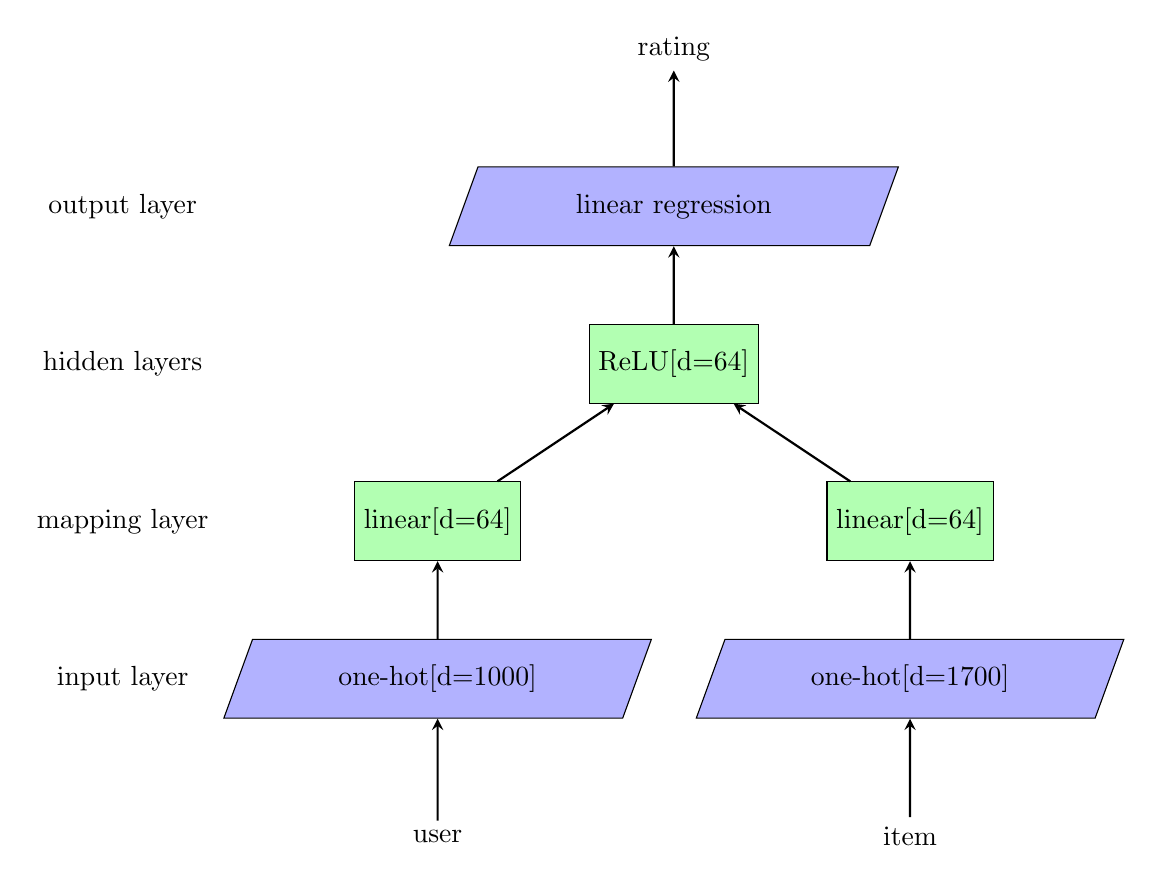
\begin{tikzpicture}[node distance=2cm]
	\tikzstyle{io} = [trapezium, trapezium left angle=70, trapezium right 
	angle=110, minimum width=1cm, minimum height=1cm, text centered, 
	draw=black, fill=blue!30]
	\tikzstyle{process} = [rectangle, minimum width=1cm, minimum height=1cm, 
	text centered, draw=black, fill=green!30]
	\tikzstyle{arrow} = [thick,->,>=stealth]
	\node (linearRegression) [io] {linear regression};
	\node (relu3) [process, below of=linearRegression] {ReLU[d=64]};
	\node (linear1) [process, below of=relu3, xshift=-3cm] {linear[d=64]};
	\node (linear2) [process, below of=relu3, xshift=3cm] {linear[d=64]};
	\node (oneHot2) [io, below of=linear2] {one-hot[d=1700]};
	\node (oneHot1) [io, below of=linear1] {one-hot[d=1000]};
	\node (rating) [above of=linearRegression] {rating};
	\node (output) [left of=linearRegression, xshift=-5cm] {output layer};
	\node (hidden1) [below of=output] {hidden layers};
	\node (mapping) [below of=hidden1] {mapping layer};
	\node (input) [below of=mapping] {input layer};
	\node (user) [below of=oneHot1] {user};
	\node (item) [below of=oneHot2] {item};
	\draw [arrow] (user) -- (oneHot1);
	\draw [arrow] (item) -- (oneHot2);
	\draw [arrow] (oneHot1) -- (linear1);
	\draw [arrow] (oneHot2) -- (linear2);
	\draw [arrow] (linear1) -- (relu3);
	\draw [arrow] (linear2) -- (relu3);
	\draw [arrow] (relu3) -- (linearRegression);
	\draw [arrow] (linearRegression) -- (rating);
	\end{tikzpicture}
	\caption{The conceptual model R for a dataset with 1700 items and 1000 
		users:
		The d in the bracket (d as in dimension) is the layer's size (number of 
		units in the layer).
		We keep all non-input layers the same size for simplicity, although 
		layers of different sizes have shown better results.
		The text before the bracket refers to the activation function of the 
		units in the layer.
		Only layers and their connections are shown, while the units in each 
		layer and their connections are not shown.
	}
	\label{fig:conceptural}
\end{figure*}
The model contains the following layers:
\begin{itemize}
	\item An input layer with one-hot activations.
	It has 1 channel for items and 1 channel for users.
	This layer is directly activated by the testing program (
	e.g., to feed the 1200th item, the testing program sets 1 at the 1200th 
	unit and 0 at other units in the item channel).
	\item A mapping layer with linear units. It has one channel to map each 
	entity to a vector.
	The activations of these two channels are the two vectors.
	It is the most critical layer as it gradually learns to map users and 
	items to vectors,
	which are complex and unobservable user and item attributes.
	\item Multiple fully connected hidden layers (only one layer is shown in the
	figure, but	multiple numbers of layers and layer sizes are evaluated in 
	the experiments) of ReLU (rectified linear units).
	These units have non-linear activation functions to give the model 
	sufficient complexity.
	These layers learn to extract more and more abstract rating-relevant 
	information.
	\item An output layer with a linear regression unit.
	It learns to predict the rating based on abstracted information.
\end{itemize}
In this problem, ratings provide the information about users and items.
We fully take this property into account and design this model to learn 
complex and unobservable user and item attributes (i.e., user and item vectors) 
supervised by a simple observable rating.

\subsection{Actual deep learning model}
In practice, Model R uses more efficient mapping tables instead of a 
one-hot input layer in order to handle a dataset with an increasing number of 
users and items, as shown in Figure \ref{fig:actural}.
The actual model has two modifications from the conceptual model:
\begin{itemize}
	\item The input layer is replaced by two mapping tables: one for users and 
	one for items.
	Their inputs are user and item IDs and their outputs are user and item 
	vectors.
	\item The mapping layer is replaced by a 2-channel input layer. It is 
	directly activated by the outputs of the mapping tables.
	\item If we need to add a new user or item into the dataset
	after the model finishes learning,
	we can add the new entry into the table and let the model learn
	only the new user or item vector using the newly introduced data,
	by fixing all other weights in the model.
	In this way the model can avoid relearning on the entire dataset.
\end{itemize}
\begin{figure*}[!ht]
	\centering
	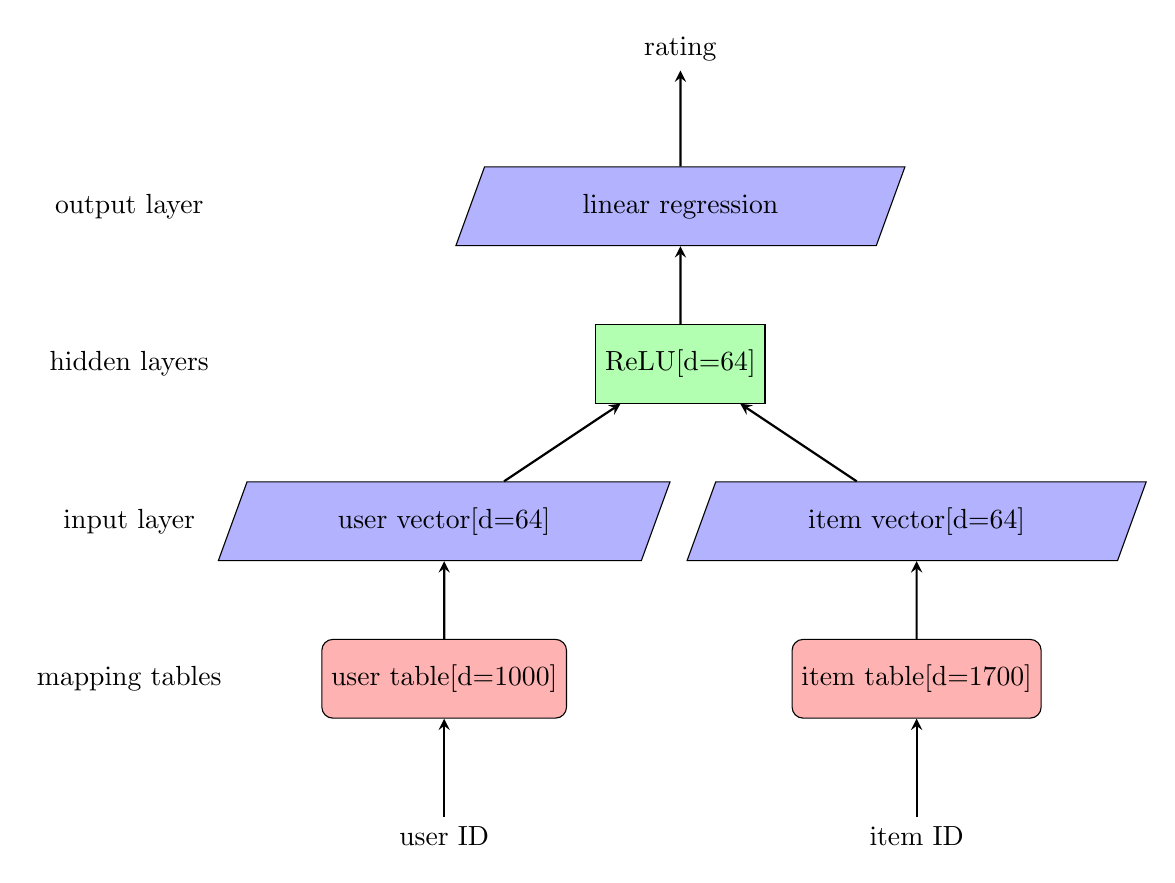
\begin{tikzpicture}[node distance=2cm]
	\tikzstyle{io} = [trapezium, trapezium left angle=70, trapezium right 
	angle=110, minimum width=1cm, minimum height=1cm, text centered, 
	draw=black, fill=blue!30]
	\tikzstyle{startstop} = [rectangle, rounded corners, minimum width=1cm, 
	minimum height=1cm, text centered, draw=black, fill=red!30]
	\tikzstyle{process} = [rectangle, minimum width=1cm, minimum height=1cm, 
	text centered, draw=black, fill=green!30]
	\tikzstyle{arrow} = [thick,->,>=stealth]
	\node (linearRegression) [io] {linear regression};
	\node (relu3) [process, below of=linearRegression] {ReLU[d=64]};
	\node (linear1) [io, below of=relu3, xshift=-3cm] {user vector[d=64]};
	\node (linear2) [io, below of=relu3, xshift=3cm] {item vector[d=64]};
	\node (oneHot1) [startstop, below of=linear1] {user table[d=1000]};
	\node (oneHot2) [startstop, below of=linear2] {item table[d=1700]};
	\node (rating) [above of=linearRegression] {rating};
	\node (output) [left of=linearRegression, xshift=-5cm] {output layer};
	\node (hidden1) [below of=output] {hidden layers};
	\node (input) [below of=hidden1] {input layer};
	\node (mapping) [below of=input] {mapping tables};
	\node (user) [below of=oneHot1] {user ID};
	\node (item) [below of=oneHot2] {item ID};
	\draw [arrow] (user) -- (oneHot1);
	\draw [arrow] (item) -- (oneHot2);
	\draw [arrow] (oneHot1) -- (linear1);
	\draw [arrow] (oneHot2) -- (linear2);
	\draw [arrow] (linear1) -- (relu3);
	\draw [arrow] (linear2) -- (relu3);
	\draw [arrow] (relu3) -- (linearRegression);
	\draw [arrow] (linearRegression) -- (rating);
	\end{tikzpicture}
	\caption{The actual model with two modifications:
		We factor the entity vector mapping process out of the neural net into 
		two mapping tables.
		We feed every item or user to the estimator by feeding their ID.
		During learning, the estimator updates the vectors in the tables the 
		same way it updates weights in the conceptual model.}
	\label{fig:actural}
\end{figure*}

\subsection{Learning techniques}
The estimator uses the above model and a number of popular deep learning 
techniques:
\begin{itemize}
	\item Backpropagation: propagation of the error gradients from output layer 
	back to each earlier layer \cite{rumelhart1988learning}
	\item Stochastic gradient descent: the optimization that minimizes 
	the error (descending against the error gradient in weight space) for a 
	random sample in each gradient decent step \cite{lecun2012efficient}
	\item Mini-batch: the modification to stochastic gradient descent to 
	accelerate and smooth the descent by minimizing the error for a small 
	random batch of samples in each gradient decent step \cite{mairal2010online}
\end{itemize}

\section{Experiments}
We evaluated Model R and the baseline solutions experimentally,
and the results show that Model R achieved much lower prediction error than 
the baseline solutions.

\subsection{Experiment settings}
We evaluated Model R in the same settings used in a recent experimental 
evaluation of the baseline solutions \cite{polatidis2016multi} on four datasets:
\begin{itemize}
	\item ML100K: MovieLens100K \cite{harper2015movielens}
	\item ML1M: MovieLens1M \cite{harper2015movielens}
	\item EP: Epinions \cite{massa2007trust}
	\item MT: MovieTweetings \cite{dooms2013movietweetings}
\end{itemize}
The specifications of the datasets are summarized in Table \ref{tab:dataset}.
The experiments use MAE as the prediction accuracy metric,
and split each dataset randomly into 2 parts: 20\% into the test set and 80\% 
into the training set.
\begin{table}[!ht]
	\centering
	\caption{The dataset specs: 
		The three columns are the dataset, number of users, items and ratings 
		of the dataset.
	}
	\begin{tabular}{cccc}  \hline
		Dataset & Users   & Items   & Ratings \\ \hline
		ML100K  & 1,000   & 1,700   & 100,000 \\ \hline
		ML1M    & 6,000   & 4,000   & 1,000,000 \\ \hline
		EP      & 49,290  & 139,738 & 664,824 \\ \hline
		MT      & 39,363  & 22,610  & 431,780 \\ \hline
	\end{tabular}
	\label{tab:dataset}
\end{table}

\subsection{Experiment process}
At the beginning of an experiment on a dataset,
the estimator sets aside 10\% of the training set as a validation set.
A larger or smaller validation set did not reduce the prediction error in the 
experiments.
Then the estimator learns for several epochs:
in each epoch,
it learns on the training set,
predicts on the validation set,
and logs the validation error.
In order to reduce over-fitting,
the estimator stops learning when the validation error has not decreased for 3 
epochs.
At the end, the testing program lets the estimator predict on the test set 
and record its testing error as its prediction error on that dataset.

\subsection{Experiment results}
In our experiments, Model R's prediction error is 18\% to 8\% lower than
the best baseline solution (i.e., MPCC) on all datasets, as shown in Table 
\ref{tab:errors}.
The error reduction from MPCC to Model R is calculated as:
\begin{align*}
\delta = \frac{MPCCError - ModelRError}{MPCCError}
\end{align*}
\begin{table}[!ht]
	\centering
	\caption{The comparison of prediction errors (measured by MAE): 
		the four baseline solutions are represented by their first letters (P, W, S, M).
		Model R's (represented by letter R) prediction error is 18\% to 9\% 
		lower than the best baseline 
		solution (MPCC) on all datasets.
	}
	\begin{tabular}{ccccccc} \hline
		Dataset & P    & W    & S    & M    & R    & $ \delta $ \\ \hline
		ML100K  & 0.83 & 0.82 & 0.83 & 0.82 & 0.69 & 16\% \\ \hline
		ML1M    & 0.83 & 0.81 & 0.83 & 0.79 & 0.65 & 18\% \\ \hline
		EP      & 1.00 & 1.02 & 1.00 & 0.93 & 0.76 & 18\% \\ \hline
		MT      & 1.38 & 1.32 & 1.33 & 1.26 & 1.15 & 9\%  \\ \hline
	\end{tabular}
	\label{tab:errors}
\end{table}
Model R is also very robust in a wide range of parameter settings, shown in 
Table \ref{tab:robust}.
\begin{table}[!ht]
	\centering
	\caption{High robustness of Model R against parameter changes:
		The estimator maintains its prediction error in range [0.68, 0.73] for 
		a wide range of parameter settings. The batch size is the size of the 
		batch of samples used in a single gradient descent step.
		These experiments are on MovieLens 100K dataset with learning rate set 
		at 0.01.
	}
	\begin{tabular}{cccc}  \hline
		batch size & layer size & hidden layers \# & MAE \\ \hline
		16 & 16 & 2 & 0.714 \\ \hline
		16 & 16 & 8 & 0.710 \\ \hline
		16 & 64 & 2 & 0.687 \\ \hline
		16 & 64 & 8 & 0.706 \\ \hline
		64 & 16 & 2 & 0.703 \\ \hline
		64 & 16 & 8 & 0.724 \\ \hline
		64 & 64 & 2 & 0.703 \\ \hline
		64 & 64 & 8 & 0.713 \\ \hline
	\end{tabular}
	\label{tab:robust}
\end{table}

\subsection{Computing resources}
We ran our experiments on a Lenovo ThinkCentre M83 machine with the following specifications:
\begin{itemize}
	\item Python implementation: CPython 3.5
	\item Operating system: Ubuntu 16.10 64-bit
	\item Memory: 16 GB
	\item Processor: Intel Core i7-4770 CPU @ 3.40GHz $ \times $ 8
\end{itemize}
The program uses all 8 threads of the processor.
Each run (learning and prediction) takes 2 to 8 minutes,
depending on the dataset and parameters in the learning algorithm.
The program is coded in Python
with popular deep learning package TensorFlow \cite{abadi2016tensorflow}.

\section{Future work}
We designed Model R for the collaborative rating prediction problem,
but we would like to incorporate a content-based capability to improve its 
prediction accuracy.
For example, in order to better predict the rating a user gives to an article,
the model can append units at the mapping layer to receive a content vector 
mapped from the text of the article by another neural net.
The model can also append one unit for each numeric attribute of the user or 
item (e.g., the age of a user, the price of a product) at the mapping layer.
In this way, it will take advantage of not only relation data but also content 
data, and therefore make more accurate predictions.
We have an open source Python implementation under MIT license hosted on Github.
The main deep learning package we use is TensorFlow 
\cite{abadi2016tensorflow}.

\section{Conclusions}
Model R shows that deep learning can be successfully applied to the 
collaborative rating prediction problem
and it can achieve higher prediction accuracy than a state-of-the-art 
collaborative filtering method.
The estimator powered by Model R effectively learns complex and unobservable 
user and item attributes from simple and observable relations (i.e., users rate 
items).
The estimator learns both to map each entity to a vector, and to predict 
the rating using these vectors.

\section*{Acknowledgements}
This material is based upon work supported by Grant No.

\bibliographystyle{IEEEtran}
\bibliography{references}
\end{document}
